\PassOptionsToPackage{unicode=true}{hyperref} % options for packages loaded elsewhere
\PassOptionsToPackage{hyphens}{url}
%
\documentclass[
]{article}
\usepackage{lmodern}
\usepackage{amssymb,amsmath}
\usepackage{ifxetex,ifluatex}
\ifnum 0\ifxetex 1\fi\ifluatex 1\fi=0 % if pdftex
  \usepackage[T1]{fontenc}
  \usepackage[utf8]{inputenc}
  \usepackage{textcomp} % provides euro and other symbols
\else % if luatex or xelatex
  \usepackage{unicode-math}
  \defaultfontfeatures{Scale=MatchLowercase}
  \defaultfontfeatures[\rmfamily]{Ligatures=TeX,Scale=1}
\fi
% use upquote if available, for straight quotes in verbatim environments
\IfFileExists{upquote.sty}{\usepackage{upquote}}{}
\IfFileExists{microtype.sty}{% use microtype if available
  \usepackage[]{microtype}
  \UseMicrotypeSet[protrusion]{basicmath} % disable protrusion for tt fonts
}{}
\makeatletter
\@ifundefined{KOMAClassName}{% if non-KOMA class
  \IfFileExists{parskip.sty}{%
    \usepackage{parskip}
  }{% else
    \setlength{\parindent}{0pt}
    \setlength{\parskip}{6pt plus 2pt minus 1pt}}
}{% if KOMA class
  \KOMAoptions{parskip=half}}
\makeatother
\usepackage{xcolor}
\IfFileExists{xurl.sty}{\usepackage{xurl}}{} % add URL line breaks if available
\IfFileExists{bookmark.sty}{\usepackage{bookmark}}{\usepackage{hyperref}}
\hypersetup{
  pdftitle={Estimating the effect of luxury cabin on the chances to survive the sinking of the Titanic},
  pdfauthor={Florian Benkhalifa, Camilla Bischofberger, Max Röcker},
  pdfborder={0 0 0},
  breaklinks=true}
\urlstyle{same}  % don't use monospace font for urls
\usepackage[margin=1in]{geometry}
\usepackage{graphicx,grffile}
\makeatletter
\def\maxwidth{\ifdim\Gin@nat@width>\linewidth\linewidth\else\Gin@nat@width\fi}
\def\maxheight{\ifdim\Gin@nat@height>\textheight\textheight\else\Gin@nat@height\fi}
\makeatother
% Scale images if necessary, so that they will not overflow the page
% margins by default, and it is still possible to overwrite the defaults
% using explicit options in \includegraphics[width, height, ...]{}
\setkeys{Gin}{width=\maxwidth,height=\maxheight,keepaspectratio}
\setlength{\emergencystretch}{3em}  % prevent overfull lines
\providecommand{\tightlist}{%
  \setlength{\itemsep}{0pt}\setlength{\parskip}{0pt}}
\setcounter{secnumdepth}{-2}
% Redefines (sub)paragraphs to behave more like sections
\ifx\paragraph\undefined\else
  \let\oldparagraph\paragraph
  \renewcommand{\paragraph}[1]{\oldparagraph{#1}\mbox{}}
\fi
\ifx\subparagraph\undefined\else
  \let\oldsubparagraph\subparagraph
  \renewcommand{\subparagraph}[1]{\oldsubparagraph{#1}\mbox{}}
\fi

% set default figure placement to htbp
\makeatletter
\def\fps@figure{htbp}
\makeatother

\usepackage{dcolumn}
\usepackage{float}
\usepackage{flafter}

\title{Estimating the effect of luxury cabin on the chances to survive the
sinking of the Titanic}
\author{Florian Benkhalifa, Camilla Bischofberger, Max Röcker}
\date{3 5 2020}

\begin{document}
\maketitle

\hypertarget{introduction}{%
\subsection{Introduction}\label{introduction}}

The purpose of this paper is to assess the effect of the economic status
(class) of the cabin on the chances of survival as a passenger on the
Titanic. The fate of the R.M.S. Titanic and its passengers has captured
the attention of the whole world. There is consensus that the chances of
getting the few places in the limited number of lifeboats and surviving
the cold waters of the North Atlantic differed among social groups.
Remarkably, women rather than men survived the disaster (Hall 1986).
This was apparently due to the long time of the sinking (2.6h) that
allowed for social norms such as `women and children first' to be
established (Frey, Savage, and Torgler 2011). However, this did not
apply across cabin classes: Eyewitness reports suggest that there was a
structural disadvantage and discrimination of third-class passengers
(Diekmann 2012). Accordingly, survivors were rather from the upper cabin
classes than from lower classes (Dixon and Griffiths 2006; Frey, Savage,
and Torgler 2011; Hall 1986). Therefore, ex ante, the effect seems to be
clear -- the lower the class of a passenger, the smaller the chances for
survival. This inequality would constitute an appalling injustice and
thus, necessitates a factual verification. Fortunately, we received
passenger data from the British Board of Trade that enables us to assess
this effect. We perform a thorough analysis in the empirical framework
of a logistic regression. We find that the relationship between class
and chances of survival is best described by including additional
variables and an interaction term. We conclude that it is likely that
the effect on the survival rate might be a combination of several
factors, with economic status of the cabin being a significant one. Our
studies suggest that passengers in the first class had a significant
higher chance to sruvive than passengers in the lower classes. The
results of this study should inform our struggle for safe passages for
everyone and workers rights worldwide.

\hypertarget{data-and-descriptives}{%
\subsection{Data and descriptives}\label{data-and-descriptives}}

The dataset ``Titanic'' contains information about the survival status
of a person, gender, the economic class and the age of each passenger.
All the variables are categorical, with only the economic class having
four categories - the remaining are binary. In total there are \(2201\)
observations in the dataset. A simple summary statistic denoting the
histograms of the variables is illustrated in the left panel of figure
\ref{fig:categories}. Two imbalances in the histograms are striking:
Adults and males are obviously more present on the titanic than children
or, respectively, females. Concerning the class variable, crew member
are the most prominent category in the dataset followed by the third
class. Since the purpose of the paper is to investigate the effect of
class on the survival rate, a preliminary grasp of the relation between
the regressors and the target variable is provided in form of several
stacked barplots in the right panel of Figure \ref{fig:categories}. They
graphically indicate differences in the survival rate between multiple
groups. The white dotted line marks the overall mean survivals and
facilitates to detect conspicious groups.

\begin{figure}[h]

{\centering 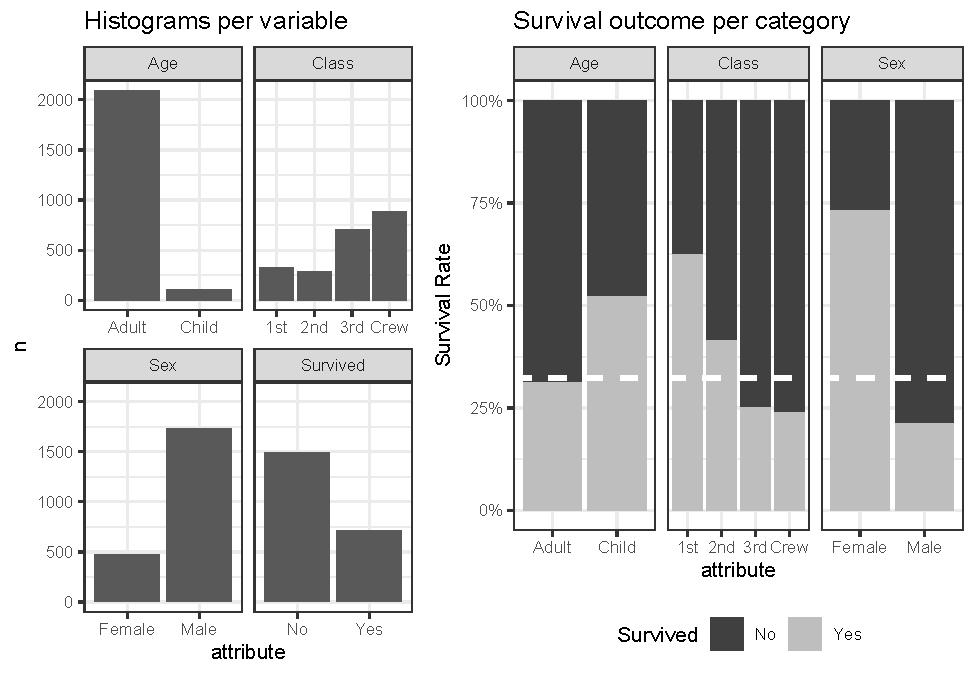
\includegraphics{Project-5_files/figure-latex/categories-1} 

}

\caption{Descriptive figures}\label{fig:categories}
\end{figure}

The graph underlines three provisional findings: (1) Children had a
higher chance to survive than adults, (2) survival rate diminishes with
economic class and (3) females were more likely to survive the crash
than males.

From a first glance the preliminary findings seem to be linked to
traditional shipping conducts. Findings 1 and 3 mostly follow from the
``Women and children first'' policy which priorises the lives of women
and children in life threatening situations. In turn it is not
surprising that male passengers reveal a low survival rate of less than
20\%. Finding (2) would lead into the direction of the presumption about
inequality among the classes described in the introduction. Thus,
validating finding 2 is of crucial interest in the next section.

\hypertarget{empirical-strategy-and-results}{%
\subsection{Empirical strategy and
results}\label{empirical-strategy-and-results}}

In this section we estimate the causal effect of the economic status of
the cabine on the chances of survival. We start with the simplest form
of logistic regression model applicable to the data which takes the form

\[P(Survived = 1|x)= G(\beta_o + \beta_1Class1 + \beta_2Class2 + \beta_3Class3) + u\]
where \(i\) denotes the i-th individual and \(\beta_0\), \(\beta_1\),
\(\beta_2\) and \(\beta_3\) are the unknown coefficients to be
estimated. \(u\) is the error of the regression and remains unobserved.
Here, the variable \(Survived\) is a binary variable indicating whether
a person survived \((Survived = 1)\) or not. The role of \(G\), which is
the logit transformation, is to keep the probability \(P(Survived = 1)\)
in between zero and one. The effect of interest is captured by the beta
coefficients which denote the impact of log odds when the survival
probability of survival of a passenger belonging to the luxury class is
compared to a lower one.

We abstain from constructing this model via a linear relationship, as
assumed by OLS, since for some range of the covariates the estimated
conditional probability may fall outside of \([0,1]\). Clearly, such
estimations violate the premise of probability functions. Further, a
linear probability model implies that a ceteris paribus increase in
\(x_i\) always corresponds with a constant change of
\(P[Survival=1|x_i]\) regardless of the initial value of \(x_i\). This
also implies that we can get \(P[Survival=1|x_i]\) greater or less than
\([0,1]\). Particularly when trying to estimate partial effects for
unseen combinations of \(x\), this should cause concerns.

Not only the dependent variable is categorical, all explenatory are
categorical as well. To account for this paper's purpose, namely to
investigate the effect of the luxury class on the chances of survival,
the explanatory variables are converted into three dummy variables. This
allows to directly compare between luxury and lower classes. In the
simple model, we have chosen to have the first class as base group. The
effect of being part of the first class is depicted in \(\beta_0\).
Consequently, \(\beta_1\), \(\beta_2\) and \(\beta_3\) depict the
increase or decrease of the survival probabilities in comparison with
the base group and the p-values denote if this difference is indeed
significant.

The estimation results of this simple model are displayed in the first
column of table 1. Table 1 contains all models we investigated in the
wake of our cross validation framework which will be explained later.

\begin{table}[t] \centering 
  \caption{Results} 
  \label{} 
\small 
\begin{tabular}{@{\extracolsep{-24pt}}lD{.}{.}{-3} D{.}{.}{-3} D{.}{.}{-3} D{.}{.}{-3} D{.}{.}{-3} D{.}{.}{-3} D{.}{.}{-3} D{.}{.}{-3} } 
\\[-1.8ex]\hline 
\hline \\[-1.8ex] 
 & \multicolumn{8}{c}{\textit{Dependent variable:}} \\ 
\cline{2-9} 
\\[-1.8ex] & \multicolumn{8}{c}{Survived} \\ 
\\[-1.8ex] & \multicolumn{1}{c}{(1)} & \multicolumn{1}{c}{(2)} & \multicolumn{1}{c}{(3)} & \multicolumn{1}{c}{(4)} & \multicolumn{1}{c}{(5)} & \multicolumn{1}{c}{(6)} & \multicolumn{1}{c}{(7)} & \multicolumn{1}{c}{(8)}\\ 
\hline \\[-1.8ex] 
 Constant & 0.509^{***} & 2.068^{***} & 0.493^{***} & 0.500^{***} & 2.044^{***} & 2.172^{***} & 0.495^{***} & 2.182^{***} \\ 
  & (0.115) & (0.168) & (0.115) & (0.115) & (0.168) & (0.174) & (0.115) & (0.176) \\ 
  & & & & & & & & \\ 
 Class\_X2nd & -0.856^{***} & -0.953^{***} & -0.932^{***} & -0.875^{***} & -1.018^{***} & -1.037^{***} & -0.940^{***} & -1.034^{***} \\ 
  & (0.166) & (0.194) & (0.168) & (0.167) & (0.196) & (0.199) & (0.168) & (0.200) \\ 
  & & & & & & & & \\ 
 Class\_X3rd & -1.596^{***} & -1.658^{***} & -1.725^{***} & -1.641^{***} & -1.778^{***} & -1.816^{***} & -1.725^{***} & -1.810^{***} \\ 
  & (0.144) & (0.168) & (0.148) & (0.145) & (0.172) & (0.175) & (0.147) & (0.176) \\ 
  & & & & & & & & \\ 
 Class\_Crew & -1.664^{***} & -0.881^{***} & -1.648^{***} & -1.655^{***} & -0.858^{***} & -0.806^{***} & -1.650^{***} & -0.803^{***} \\ 
  & (0.139) & (0.157) & (0.139) & (0.139) & (0.157) & (0.160) & (0.139) & (0.160) \\ 
  & & & & & & & & \\ 
 Sex\_Male &  & -2.421^{***} &  &  & -2.420^{***} & -2.606^{***} &  & -2.617^{***} \\ 
  &  & (0.139) &  &  & (0.140) & (0.147) &  & (0.151) \\ 
  & & & & & & & & \\ 
 Sex\_Male\_x\_Age\_Child &  &  &  & 0.699^{***} &  & 1.795^{***} & -0.711^{*} & 1.902^{***} \\ 
  &  &  &  & (0.268) &  & (0.283) & (0.406) & (0.433) \\ 
  & & & & & & & & \\ 
 Age\_Child &  &  & 1.072^{***} &  & 1.062^{***} &  & 1.490^{***} & -0.110 \\ 
  &  &  & (0.211) &  & (0.244) &  & (0.322) & (0.335) \\ 
  & & & & & & & & \\ 
\hline \\[-1.8ex] 
cv.accuracy & 0.714 & 0.776 & 0.725 & 0.719 & 0.778 & 0.783 & 0.723 & 0.783 \\ 
cv.kap & 0.235 & 0.436 & 0.273 & 0.253 & 0.443 & 0.459 & 0.278 & 0.458 \\ 
Observations & \multicolumn{1}{c}{2,201} & \multicolumn{1}{c}{2,201} & \multicolumn{1}{c}{2,201} & \multicolumn{1}{c}{2,201} & \multicolumn{1}{c}{2,201} & \multicolumn{1}{c}{2,201} & \multicolumn{1}{c}{2,201} & \multicolumn{1}{c}{2,201} \\ 
Log Likelihood & \multicolumn{1}{c}{-1,294.278} & \multicolumn{1}{c}{-1,114.456} & \multicolumn{1}{c}{-1,281.486} & \multicolumn{1}{c}{-1,290.982} & \multicolumn{1}{c}{-1,105.031} & \multicolumn{1}{c}{-1,096.075} & \multicolumn{1}{c}{-1,279.928} & \multicolumn{1}{c}{-1,096.021} \\ 
Akaike Inf. Crit. & \multicolumn{1}{c}{2,596.555} & \multicolumn{1}{c}{2,238.913} & \multicolumn{1}{c}{2,572.972} & \multicolumn{1}{c}{2,591.965} & \multicolumn{1}{c}{2,222.061} & \multicolumn{1}{c}{2,204.150} & \multicolumn{1}{c}{2,571.855} & \multicolumn{1}{c}{2,206.043} \\ 
\hline 
\hline \\[-1.8ex] 
\textit{Note:}  & \multicolumn{8}{r}{$^{*}$p$<$0.1; $^{**}$p$<$0.05; $^{***}$p$<$0.01} \\ 
 & \multicolumn{8}{r}{Standard deviations in parentheses} \\ 
\end{tabular} 
\end{table}

The constant \(\beta_0\) is the only estimate which is positive, all
other coefficients are negative. This suggests that the first class has
the highest chance of survival compared to the other classes. Being part
of the crew class seems to decrease survival chances the most. A similar
impact can be found for the third class, so being a passenger in the
third class or being a crew member reduces the chances of survival
almost equally compared to the first class passengers. Second class
members are less likely to survive than first class members but still
have better chances then the remaining classes. These findings match
what we see in our preliminary findins in figure \ref{fig:categories} -
the survival rate of the third class and the crew class are almost the
same around 25\%, followed by the second class and finally the first
class, which has the highest survival rate.

To test our hypothesis that being a passenger in the luxury class
results in the highest survival chances we define the null hypothesis as
the following. \[H_0 : \beta_i < 0 \text{ for } i =\{1,2,3\}\] We can
reject the hypothesis for all of the estimates on a 99\% confidence
bound, according to the results in table 1, with the p-values being very
close to zero. We also test for joint significance of the simple model
via a ANOVA Chi-Square.

\begin{table}[H] \centering 
  \caption{Chi-Squared for Model (1)} 
  \label{} 
\small 
\begin{tabular}{@{\extracolsep{5pt}} cccccc} 
\\[-1.8ex]\hline 
\hline \\[-1.8ex] 
 & Df & Deviance & Resid. Df & Resid. Dev & Pr(\textgreater Chi) \\ 
\hline \\[-1.8ex] 
NULL & $$ & $$ & $2,200$ & $2,769.457$ & $$ \\ 
Class\_X2nd & $1$ & $11.974$ & $2,199$ & $2,757.483$ & $0.001$ \\ 
Class\_X3rd & $1$ & $17.525$ & $2,198$ & $2,739.957$ & $0.00003$ \\ 
Class\_Crew & $1$ & $151.402$ & $2,197$ & $2,588.555$ & $0$ \\ 
\hline \\[-1.8ex] 
\end{tabular} 
\end{table}

It turns out that adding the variables sequentially to the model indeed
improves the model and hence we can conclude that the coefficients are
joint significant.

We now perform the model diagnostics. The important questions are
whether the estimates are credible and whether the assumptions behind
the simple model hold. In order to interpret the variable in a causal
manner, this simple randomized model works under two main assumptions:
First, that on average the error is zero \((E[u_i = 0])\) and second,
that there is randomization \((x \bot u)\) and thus, no correlation
between our error term and the Class variables (exogeneity). Exogeneity
can be highly questioned, since the error term might contain the other
variables gender and age which are observed in the dataset. Moreover,
factors contained in the error term could be body weight, body fat,
physical condition, swimming abilities, intelligence, clothing, number
of family members on the ship, location in the ship or the distribution
of flotsam. Those variables could simultaneously affect the class
variables and the outcome. Our data doesn't come from a randomized
experiment but we could think of a randomized experiment in order to
extract the effect of class. Therefore, we would randomly pick 1000
people representative for passengers who prefer to travel by a liner.
For instance, past passenger on different liners across the world could
be pooled into a dataset, and 1000 people are randomly chosen and
informed that they won a free a cruise in a lottery. Once they arrive on
a representative liner, they are randomly assigned to different cabin
classes. Eventually the ship is forced to sink in the Atlantic.
Fortunately, this experiment will most probably never take place.

As we have binary variables, there is no possibility to add polynomials
of higher degree to our model. In order to choose a more complex model,
we include more dummy variables as well as interaction terms between
them. We then perform a feature selection procedure by repeating a 15
fold cross validation 10 times for each possible combination of dummy
variables and interaction terms. Since the purpose of the paper still is
to estimate the effect of class on the survival rate, we force the class
dummies to be present in the dataset in each submodel and abstain from
including interaction with one of the class dummies. We collect two
metrics which are common for binary classification tasks: accuracy and
kappa statistic.Accuracy is defined as
\(\frac{\text{Number of correct predictions}}{\text{Total number of predictions}}\).
The metric can be misleading, particularly when there are class
imbalances in the outcome. With roughly 30\% of survivors this could be
an issue. To account for this problem we also include the kappa
statistic which measures the performance of a classifier independent of
class imbalances. Both values are displayed in table 1. Obviously model
(8), where all dummies and interactions are included, performs best. The
worst performance was achieved by the simple model (1). Table 1 gives
interesting insights on the size and direction of the bias. In models,
where Sex is not included, as for instance (1), (3) and (4), the class
crew has a remarkably more negative impact on surviving, compared to the
other models. This can be explained by looking at
\(P(Sex = Male|Class = Crew) = 0.97\). The number indicates that part of
the lower surviving chances of the crew members can be explained by the
overproportional share of men in that group. In all the models, the
first class remains the class with the higher survival chances.

We now turn our focus on a more thorough analysis of model (8). All
dummies and interaction terms are included and a female, adult person
from the first class was chosen as base group. The inclusion of all
available variables does not only increase the accuracy and kappa
statistic, but also renders the model's exogeneity assumption more
credible, although variables such as intelligence, muscle strength, etc,
surely still impose a bias on the estimates. All estimates except
Age\_child are significant on 99\% confidence level. Interestingly, some
coefficients change remarkably in the complex model. As already
mentionned before, the crew class now has a higher surviving strategy,
even surpassing the second class. So being part of the crew actually
poses the second best circumstance on surviving besides being in the
luxury class. Being male is obviously the highest threat for surviving
with a coefficient exceeding -2.6.

It is interesting to further investigate the insignificance of
Age\_Child. It implies, that either being female or child result in the
same chance on surviving. In other words, if a person is female, there
is no evidence that being a child boosts the surviving probability even
more. To the contrary, being a male child does increase the surviving
chance even beyond the surviving chance of a girl. This could have
several reasons, such as boys having a better swimming ability or being
quicker on foot than girls. Compared to the simple model, the class
variables have changed due to a reduced ommited varible bias. We cannot
quantify the bias since we do not know the true beta coefficients.
Because of many variables missing we also suspect the complex model to
be biased. However, we can dare to make statements about the direction
of the bias in the simple model with the \(\beta_0\) being downward
biased, \(\beta_1\) being downward biased, \(\beta_2\) being downward
biased, and \(\beta_3\) being upward biased. We conclude with a
likelihood ratio test, to ensure that our complex model performs better
than the simple.

\begin{table}[!htbp] \centering 
  \caption{Chi-Squared for Model (8)} 
  \label{} 
\small 
\begin{tabular}{@{\extracolsep{5pt}} cccccc} 
\\[-1.8ex]\hline 
\hline \\[-1.8ex] 
 & Resid. Df & Resid. Dev & Df & Deviance & Pr(\textgreater Chi) \\ 
\hline \\[-1.8ex] 
1 & $2,197$ & $2,588.555$ & $$ & $$ & $$ \\ 
2 & $2,194$ & $2,192.043$ & $3$ & $396.513$ & $0$ \\ 
\hline \\[-1.8ex] 
\end{tabular} 
\end{table}

In the table, the first model denotes the simple model which is compared
to the more complex one. The p-value is highly significant which means
that our complex model outperforms the simple model.

\hypertarget{conclusion}{%
\subsection{Conclusion}\label{conclusion}}

In summary, the economic status of the cabin (class) appears to have an
effect on the survival chances. The positive effect which a passenger in
the first class enjoys on its survival chances decreases with economic
class. However, after controlling for the gender, crew members have the
second highest probability to survive. Being a child or a female both
significantly increases the survival chances - indicating that the women
and children first policy was a successful measure on the titanic. Thus,
our findings concur with the literature. In consequence, we suggest a
policy change that makes the Atlantic passage safe for all passengers,
regardless of class. This could include raising the number of lifeboats
and life vests to a number that reflects the passenger numbers and
ensuring that lifeboats can easily be accessed from different cabin
class areas.

\newpage

\hypertarget{references}{%
\section{References}\label{references}}

\hypertarget{refs}{}
\leavevmode\hypertarget{ref-diekmann2012}{}%
Diekmann, Andreas. 2012. ``Die Rolle sozialer Normen, der
Situationsdefinition und sozialer Klassen beim Untergang der Titanic.''
\emph{KZfSS Kölner Zeitschrift Für Soziologie Und Sozialpsychologie} 64
(1): 175--84. \url{https://doi.org/10.1007/s11577-012-0160-y}.

\leavevmode\hypertarget{ref-dixon2006}{}%
Dixon, Robert, and William Griffiths. 2006. ``Survival on the Titanic:
Illustrating Wald and Lagrange Multiplier Tests for Proportions and
Logits.'' \emph{The Journal of Economic Education} 37 (3): 289--304.
\url{https://doi.org/10.3200/JECE.37.3.289-304}.

\leavevmode\hypertarget{ref-frey2011}{}%
Frey, Bruno S, David A Savage, and Benno Torgler. 2011. ``Behavior Under
Extreme Conditions: The \emph{Titanic} Disaster.'' \emph{Journal of
Economic Perspectives} 25 (1): 209--22.
\url{https://doi.org/10.1257/jep.25.1.209}.

\leavevmode\hypertarget{ref-hall1986}{}%
Hall, Wayne. 1986. ``Social Class and Survival on the S.S. Titanic.''
\emph{Social Science \& Medicine} 22 (6): 687--90.
\url{https://doi.org/10.1016/0277-9536(86)90041-9}.

\newpage

\hypertarget{appendix}{%
\section{Appendix}\label{appendix}}

\begin{table}[!htbp] \centering 
  \caption{P(Sex)} 
  \label{} 
\begin{tabular}{@{\extracolsep{5pt}} ccc} 
\\[-1.8ex]\hline 
\hline \\[-1.8ex] 
Sex & n & P(Sex) \\ 
\hline \\[-1.8ex] 
Female &  470 & 0.21 \\ 
Male & 1731 & 0.79 \\ 
\hline \\[-1.8ex] 
\end{tabular} 
\end{table}

\begin{table}[!htbp] \centering 
  \caption{P(Age)} 
  \label{} 
\begin{tabular}{@{\extracolsep{5pt}} ccc} 
\\[-1.8ex]\hline 
\hline \\[-1.8ex] 
Age & n & P(Age) \\ 
\hline \\[-1.8ex] 
Adult & 2092 & 0.95 \\ 
Child &  109 & 0.05 \\ 
\hline \\[-1.8ex] 
\end{tabular} 
\end{table}

\begin{table}[!htbp] \centering 
  \caption{P(Class)} 
  \label{} 
\begin{tabular}{@{\extracolsep{5pt}} ccc} 
\\[-1.8ex]\hline 
\hline \\[-1.8ex] 
Class & n & P(Class) \\ 
\hline \\[-1.8ex] 
1st & 325 & 0.15 \\ 
2nd & 285 & 0.13 \\ 
3rd & 706 & 0.32 \\ 
Crew & 885 & 0.40 \\ 
\hline \\[-1.8ex] 
\end{tabular} 
\end{table}

\begin{table}[!htbp] \centering 
  \caption{P(Class, Sex)} 
  \label{} 
\begin{tabular}{@{\extracolsep{5pt}} cccc} 
\\[-1.8ex]\hline 
\hline \\[-1.8ex] 
Class & Sex & n & P(Class, Sex) \\ 
\hline \\[-1.8ex] 
1st & Female & 145 & 0.07 \\ 
1st & Male & 180 & 0.08 \\ 
2nd & Female & 106 & 0.05 \\ 
2nd & Male & 179 & 0.08 \\ 
3rd & Female & 196 & 0.09 \\ 
3rd & Male & 510 & 0.23 \\ 
Crew & Female &  23 & 0.01 \\ 
Crew & Male & 862 & 0.39 \\ 
\hline \\[-1.8ex] 
\end{tabular} 
\end{table}

\begin{table}[!htbp] \centering 
  \caption{P(Class, Age)} 
  \label{} 
\begin{tabular}{@{\extracolsep{5pt}} cccc} 
\\[-1.8ex]\hline 
\hline \\[-1.8ex] 
Class & Age & n & P(Class, Age) \\ 
\hline \\[-1.8ex] 
1st & Adult & 319 & 0.14 \\ 
1st & Child &   6 & 0.00 \\ 
2nd & Adult & 261 & 0.12 \\ 
2nd & Child &  24 & 0.01 \\ 
3rd & Adult & 627 & 0.28 \\ 
3rd & Child &  79 & 0.04 \\ 
Crew & Adult & 885 & 0.40 \\ 
Crew & Child &   0 & 0.00 \\ 
\hline \\[-1.8ex] 
\end{tabular} 
\end{table}

\begin{table}[!htbp] \centering 
  \caption{P(Sex|Class)} 
  \label{} 
\begin{tabular}{@{\extracolsep{5pt}} cccc} 
\\[-1.8ex]\hline 
\hline \\[-1.8ex] 
Class & Sex & n & P(Sex\textbar Class) \\ 
\hline \\[-1.8ex] 
1st & Female & 145 & 0.45 \\ 
1st & Male & 180 & 0.55 \\ 
2nd & Female & 106 & 0.37 \\ 
2nd & Male & 179 & 0.63 \\ 
3rd & Female & 196 & 0.28 \\ 
3rd & Male & 510 & 0.72 \\ 
Crew & Female &  23 & 0.03 \\ 
Crew & Male & 862 & 0.97 \\ 
\hline \\[-1.8ex] 
\end{tabular} 
\end{table}

\begin{table}[!htbp] \centering 
  \caption{P(Class|Sex)} 
  \label{} 
\begin{tabular}{@{\extracolsep{5pt}} cccc} 
\\[-1.8ex]\hline 
\hline \\[-1.8ex] 
Class & Sex & n & P(Class\textbar Sex) \\ 
\hline \\[-1.8ex] 
1st & Female & 145 & 0.31 \\ 
1st & Male & 180 & 0.10 \\ 
2nd & Female & 106 & 0.23 \\ 
2nd & Male & 179 & 0.10 \\ 
3rd & Female & 196 & 0.42 \\ 
3rd & Male & 510 & 0.29 \\ 
Crew & Female &  23 & 0.05 \\ 
Crew & Male & 862 & 0.50 \\ 
\hline \\[-1.8ex] 
\end{tabular} 
\end{table}

\begin{table}[!htbp] \centering 
  \caption{P(Sex|Age)} 
  \label{} 
\begin{tabular}{@{\extracolsep{5pt}} cccc} 
\\[-1.8ex]\hline 
\hline \\[-1.8ex] 
Sex & Age & n & P(Sex\textbar Age) \\ 
\hline \\[-1.8ex] 
Female & Adult &  425 & 0.20 \\ 
Male & Adult & 1667 & 0.80 \\ 
Female & Child &   45 & 0.41 \\ 
Male & Child &   64 & 0.59 \\ 
\hline \\[-1.8ex] 
\end{tabular} 
\end{table}

\begin{table}[!htbp] \centering 
  \caption{Chi-Squared for Model (1)} 
  \label{} 
\small 
\begin{tabular}{@{\extracolsep{5pt}} cccccc} 
\\[-1.8ex]\hline 
\hline \\[-1.8ex] 
 & Df & Deviance & Resid. Df & Resid. Dev & Pr(\textgreater Chi) \\ 
\hline \\[-1.8ex] 
NULL & $$ & $$ & $2,200$ & $2,769.457$ & $$ \\ 
Sex\_Male & $1$ & $434.469$ & $2,199$ & $2,334.988$ & $0$ \\ 
Age\_Child & $1$ & $5.893$ & $2,198$ & $2,329.095$ & $0.015$ \\ 
Sex\_Male\_x\_Age\_Child & $1$ & $16.319$ & $2,197$ & $2,312.776$ & $0.0001$ \\ 
Class\_X2nd & $1$ & $0.069$ & $2,196$ & $2,312.707$ & $0.793$ \\ 
Class\_X3rd & $1$ & $95.778$ & $2,195$ & $2,216.929$ & $0$ \\ 
Class\_Crew & $1$ & $24.887$ & $2,194$ & $2,192.043$ & $0.00000$ \\ 
\hline \\[-1.8ex] 
\end{tabular} 
\end{table}

```

\end{document}
